\documentclass{article}

% content/resources/templates/preamble.tex
\usepackage[margin=0.6in]{geometry}
\author{Milav Dabgar}
\usepackage{amsmath,amssymb,amsthm}
\usepackage{booktabs}
\usepackage{multirow}
\usepackage{xcolor}
\usepackage{tcolorbox}
\tcbuselibrary{breakable,skins}
\usepackage[colorlinks=true,linkcolor=blue]{hyperref}
\usepackage{titlesec}
\usepackage{enumitem}
\usepackage{tikz}
\usepackage{pgfplots}
\usepackage{circuitikz}
\usepackage[version=4]{mhchem}
\usepackage{longtable}
\usepackage{array}
\usepackage{float}
\usepackage{caption}
\usepackage{listings}

\lstset{
  basicstyle=\small\ttfamily,
  breaklines=true,
  breakatwhitespace=false,
  postbreak=\mbox{\textcolor{red}{$\hookrightarrow$}\space},
  float=false,
  numbers=left,
  numberstyle=\tiny\color{gray},
  numbersep=10pt,
  xleftmargin=2em,
  keywordstyle=\color{blue},
  commentstyle=\color{green!60!black},
  stringstyle=\color{purple},
  backgroundcolor=\color{gray!5},
  showstringspaces=false,
  tabsize=2,
  captionpos=b,
  keepspaces=true,
  columns=flexible
}

\pgfplotsset{compat=1.18}
\usetikzlibrary{shapes,arrows,positioning,calc,patterns,decorations.pathmorphing,decorations.markings,arrows.meta}

% Color scheme
\definecolor{headcolor}{RGB}{0,102,204}
\definecolor{keycolor}{RGB}{220,20,60}
\definecolor{solutioncolor}{RGB}{34,139,34}
\definecolor{mnemoniccolor}{RGB}{148,0,211}
\definecolor{codecolor}{RGB}{0,0,100}

% Spacing
\setlength{\parskip}{3pt}
\setlist[itemize]{nosep}
\setlist[enumerate]{nosep}

% Title formatting
\titleformat{\section}{\Large\bfseries\color{headcolor}}{\thesection}{1em}{}
\titleformat{\subsection}{\large\bfseries\color{headcolor}}{\thesubsection}{1em}{}

% Pandoc tightlist compatibility
\providecommand{\tightlist}{%
  \setlength{\itemsep}{0pt}\setlength{\parskip}{0pt}}

% Pandoc longtable compatibility
\newcounter{none}
\def\thenone{}


% Custom commands for GTU solutions
% This file defines semantic commands for consistent formatting

% Question command with automatic formatting
\newcommand{\question}[2]{%
  \section*{Question #1}%
  \textbf{#2}%
}

% OR question variant
\newcommand{\questionor}[2]{%
  \section*{Question #1 OR}%
  \textbf{#2}%
}

% Proper table environment with caption
\newenvironment{answertable}[1]{%
  \begin{table}[htbp]
  \centering
  \caption{#1}
}{%
  \end{table}
}

% Proper figure environment for diagrams
\newenvironment{answerdiagram}[1]{%
  \begin{figure}[htbp]
  \centering
  \caption{#1}
}{%
  \end{figure}
}

% Semantic markup for key terms
\newcommand{\keyword}[1]{\textbf{#1}}
\newcommand{\code}[1]{\texttt{#1}}
\newcommand{\classname}[1]{\texttt{#1}}
\newcommand{\methodname}[1]{\texttt{#1}}

% Proper quotation marks
\newcommand{\mnemonic}[1]{``#1''}


% content/resources/templates/english-boxes.tex
% This file is currently empty - it exists to maintain consistency with the import structure.
% Add custom environments here if needed in the future.


% Redefine environments to be non-floating for tcolorbox compatibility
\renewenvironment{answertable}[1]{%
  \begin{center}
  \captionof{table}{#1}
}{%
  \end{center}
}

\renewenvironment{answerdiagram}[1]{%
  \begin{center}
  \captionof{figure}{#1}
}{%
  \end{center}
}

\title{Cyber Security (4353204) - Summer 2025 Solution}
\date{May 16, 2025}

\begin{document}
\maketitle

% Question 1
\questionmarks{1(a)}{3}{Describe CIA triad with example.}

\begin{solutionbox}
\textbf{CIA Triad Components:}

\begin{answerdiagram}{CIA Triad}
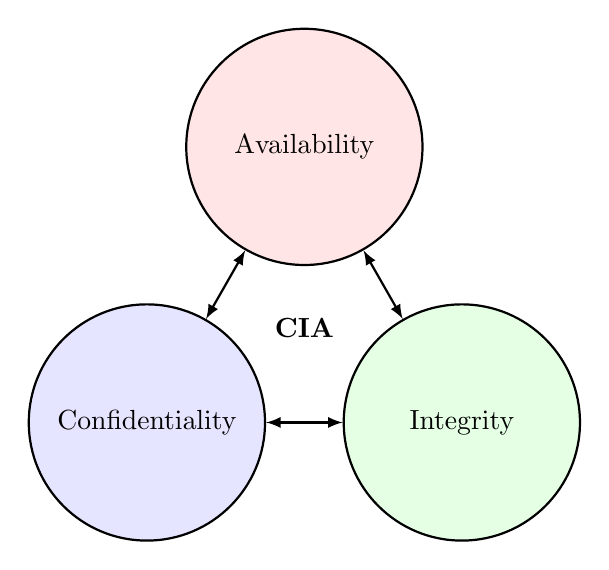
\begin{tikzpicture}[node distance=2.5cm, auto, >=latex, thick]
    % Nodes
    \node [draw, circle, minimum size=3cm, align=center, fill=blue!10] (conf) {Confidentiality};
    \node [draw, circle, minimum size=3cm, align=center, fill=green!10] (int) at (4,0) {Integrity};
    \node [draw, circle, minimum size=3cm, align=center, fill=red!10] (avail) at (2,3.5) {Availability};
    
    % Connections
    \draw [<->] (conf) -- (int);
    \draw [<->] (int) -- (avail);
    \draw [<->] (avail) -- (conf);
    
    % Center label
    \node at (2,1.2) {\textbf{CIA}};
\end{tikzpicture}
\end{answerdiagram}

\begin{answertable}{CIA Triad Elements}
\begin{tabulary}{\linewidth}{|L|L|L|}
\hline
\textbf{Component} & \textbf{Definition} & \textbf{Example} \\ \hline
\keyword{Confidentiality} & Protecting data from unauthorized access & Password protection on bank accounts \\ \hline
\keyword{Integrity} & Ensuring data accuracy and completeness & Digital signatures on documents \\ \hline
\keyword{Availability} & Ensuring systems are accessible when needed & 24/7 online banking services \\ \hline
\end{tabulary}
\end{answertable}

\begin{itemize}
    \item \keyword{Confidentiality}: Only authorized users can access sensitive information
    \item \keyword{Integrity}: Data remains accurate and unaltered during transmission
    \item \keyword{Availability}: Systems remain operational and accessible to legitimate users
\end{itemize}
\end{solutionbox}

\begin{mnemonicbox}
\mnemonic{CIA Keeps Information Safe}
\end{mnemonicbox}

\questionmarks{1(b)}{4}{Explain Public key and Private Key cryptography.}

\begin{solutionbox}
\textbf{Public Key Cryptography (Asymmetric):}

\begin{answerdiagram}{Public Key Cryptography Flow}
\begin{tikzpicture}[auto, >=latex, thick, node distance=2cm]
    \node [gtu state] (sender) {Sender};
    \node [gtu block, right=of sender] (encrypt) {Encrypt};
    \node [right=of encrypt] (network) {Network};
    \node [gtu block, right=of network] (decrypt) {Decrypt};
    \node [gtu state, right=of decrypt] (receiver) {Receiver};
    
    % Keys
    \node [above=0.5cm of encrypt, draw, rectangle, fill=yellow!20] (pubkey) {Receiver's Public Key};
    \node [above=0.5cm of decrypt, draw, rectangle, fill=red!20] (privkey) {Receiver's Private Key};
    
    % Connections
    \draw [gtu arrow] (sender) -- node {Plaintext} (encrypt);
    \draw [gtu arrow] (pubkey) -- (encrypt);
    \draw [gtu arrow] (encrypt) -- node {Ciphertext} (decrypt);
    \draw [gtu arrow] (privkey) -- (decrypt);
    \draw [gtu arrow] (decrypt) -- node {Plaintext} (receiver);
\end{tikzpicture}
\end{answerdiagram}

\textbf{Key Characteristics:}

\begin{answertable}{Public vs Private Key}
\begin{tabulary}{\linewidth}{|L|L|L|}
\hline
\textbf{Feature} & \textbf{Public Key} & \textbf{Private Key} \\ \hline
\textbf{Distribution} & Freely shared & Kept secret \\ \hline
\textbf{Usage} & Encryption/Verification & Decryption/Signing \\ \hline
\textbf{Security} & Can be public & Must be protected \\ \hline
\end{tabulary}
\end{answertable}

\begin{itemize}
    \item \keyword{Public Key}: Used for encryption and signature verification
    \item \keyword{Private Key}: Used for decryption and digital signing
    \item \keyword{Security}: Based on mathematical complexity (RSA, ECC algorithms)
\end{itemize}
\end{solutionbox}

\begin{mnemonicbox}
\mnemonic{Public Encrypts, Private Decrypts}
\end{mnemonicbox}

\questionmarks{1(c)}{7}{Explain various security attacks, mechanisms, and services associated with each layer of the OSI model.}

\begin{solutionbox}
\textbf{OSI Security Framework:}

\begin{answerdiagram}{OSI Security Framework}
\begin{tikzpicture}[
    layer/.style={draw, rectangle, minimum width=4cm, minimum height=0.8cm, fill=blue!5, align=center},
    attack/.style={draw, rectangle, minimum width=4cm, minimum height=0.8cm, fill=red!5, align=center, font=\footnotesize},
    mech/.style={draw, rectangle, minimum width=4cm, minimum height=0.8cm, fill=green!5, align=center, font=\footnotesize}
]
    % OSI Layers
    \node[layer] (app) {Application};
    \node[layer, below=0.1cm of app] (pres) {Presentation};
    \node[layer, below=0.1cm of pres] (sess) {Session};
    \node[layer, below=0.1cm of sess] (trans) {Transport};
    \node[layer, below=0.1cm of trans] (net) {Network};
    \node[layer, below=0.1cm of net] (link) {Data Link};
    \node[layer, below=0.1cm of link] (phy) {Physical};
    
    % Attacks (Left)
    \node[attack, left=1cm of app] {Malware, Social Eng.};
    \node[attack, left=1cm of pres] {Format attacks};
    \node[attack, left=1cm of sess] {Hijacking};
    \node[attack, left=1cm of trans] {SYN Flooding};
    \node[attack, left=1cm of net] {IP Spoofing};
    \node[attack, left=1cm of link] {MAC Flooding};
    \node[attack, left=1cm of phy] {Wiretapping};
    
    % Mechanisms (Right)
    \node[mech, right=1cm of app] {Antivirus};
    \node[mech, right=1cm of pres] {Encryption};
    \node[mech, right=1cm of sess] {Tokens};
    \node[mech, right=1cm of trans] {SSL/TLS};
    \node[mech, right=1cm of net] {IPSec/Firewall};
    \node[mech, right=1cm of link] {Auth/Encryption};
    \node[mech, right=1cm of phy] {Shielding};
    
    % Labels
    \node[above=0.2cm of app] {\textbf{OSI Layer}};
    \node[above=0.2cm of app, xshift=-5cm] {\textbf{Attacks}};
    \node[above=0.2cm of app, xshift=5cm] {\textbf{Mechanisms}};
    
    % Connectors (optional, can just align)
    \draw[dashed, gray] (app) -- (mech, right=1cm of app);
\end{tikzpicture}
\end{answerdiagram}

\begin{answertable}{OSI Layers Security Details}
\begin{tabulary}{\linewidth}{|L|L|L|L|}
\hline
\textbf{Layer} & \textbf{Attacks} & \textbf{Mechanisms} & \textbf{Services} \\ \hline
\keyword{Physical} & Wiretapping, Jamming & Physical security, Shielding & Access control \\ \hline
\keyword{Data Link} & MAC flooding, ARP poisoning & Encryption, Authentication & Frame integrity \\ \hline
\keyword{Network} & IP spoofing, Routing attacks & IPSec, Firewalls & Packet filtering \\ \hline
\keyword{Transport} & Session hijacking, SYN flooding & SSL/TLS, Port security & End-to-end security \\ \hline
\keyword{Session} & Session replay, Hijacking & Session tokens, Timeouts & Session management \\ \hline
\keyword{Presentation} & Data corruption, Format attacks & Encryption, Compression & Data transformation \\ \hline
\keyword{Application} & Malware, Social engineering & Antivirus, User training & Application security \\ \hline
\end{tabulary}
\end{answertable}

\textbf{Key Security Services:}
\begin{itemize}
    \item \keyword{Authentication}: Verifying user identity
    \item \keyword{Authorization}: Controlling access permissions
    \item \keyword{Non-repudiation}: Preventing denial of actions
    \item \keyword{Data integrity}: Ensuring data accuracy
\end{itemize}
\end{solutionbox}

\begin{mnemonicbox}
\mnemonic{All People Seem To Need Data Protection}
\end{mnemonicbox}

\questionmarks{1(c OR)}{7}{Explain MD5 hashing and Secure Hash Function (SHA) algorithms.}

\begin{solutionbox}
\textbf{Hash Function Comparison:}

\begin{answerdiagram}{Hash Function Process}
\begin{tikzpicture}[auto, >=latex, thick, node distance=1.5cm]
    \node [gtu block, minimum width=2.5cm] (input) {Input Message\\(Any Length)};
    \node [gtu block, right=1cm of input, minimum width=2.5cm, fill=orange!10] (hash) {Hash Function\\(MD5/SHA)};
    \node [gtu block, right=1cm of hash, minimum width=2.5cm, fill=green!10] (digest) {Fixed-Size Hash\\(Digital Fingerprint)};
    
    \draw [gtu arrow] (input) -- (hash);
    \draw [gtu arrow] (hash) -- (digest);
    
    \node [below=0.5cm of hash, align=center, font=\small] {Deterministic\\One-way};
\end{tikzpicture}
\end{answerdiagram}

\begin{answertable}{MD5 vs SHA Comparison}
\begin{tabulary}{\linewidth}{|L|L|L|L|}
\hline
\textbf{Feature} & \textbf{MD5} & \textbf{SHA-1} & \textbf{SHA-256} \\ \hline
\textbf{Output Size} & 128 bits & 160 bits & 256 bits \\ \hline
\textbf{Security Level} & Weak & Weak & Strong \\ \hline
\textbf{Speed} & Fast & Moderate & Slower \\ \hline
\textbf{Current Status} & Deprecated & Deprecated & Recommended \\ \hline
\end{tabulary}
\end{answertable}

\textbf{Hash Properties:}
\begin{itemize}
    \item \keyword{Deterministic}: Same input produces same hash
    \item \keyword{Avalanche Effect}: Small input change causes major hash change
    \item \keyword{One-way Function}: Cannot reverse hash to original data
    \item \keyword{Collision Resistant}: Difficult to find two inputs with same hash
\end{itemize}

\textbf{Applications:}
\begin{itemize}
    \item Password storage and verification
    \item Digital signatures and certificates
    \item Data integrity verification
\end{itemize}
\end{solutionbox}

\begin{mnemonicbox}
\mnemonic{Hash Always Produces Same Output}
\end{mnemonicbox}

% Question 2
\questionmarks{2(a)}{3}{What is firewall? List out types of firewall.}

\begin{solutionbox}
\textbf{Firewall Definition:}
Network security device that monitors and controls incoming/outgoing traffic based on security rules.

\begin{answerdiagram}{Firewall Architecture}
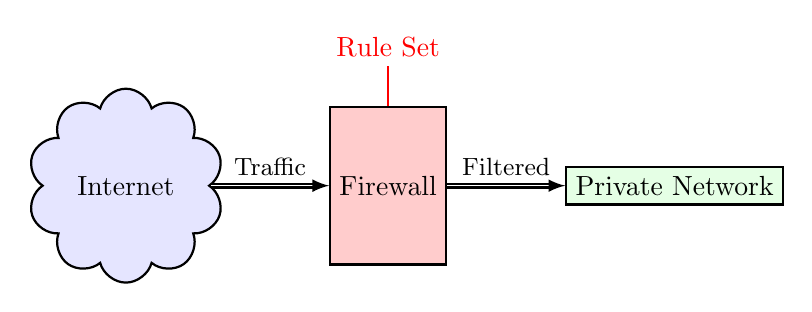
\begin{tikzpicture}[auto, >=latex, thick]
    \node [draw, cloud, cloud puffs=10, minimum width=2.5cm, fill=blue!10] (internet) {Internet};
    \node [draw, rectangle, fill=red!20, minimum height=2cm, right=1.5cm of internet] (firewall) {Firewall};
    \node [draw, rectangle, fill=green!10, right=1.5cm of firewall] (lan) {Private Network};
    
    \draw [->, double] (internet) -- node[above, font=\small] {Traffic} (firewall);
    \draw [->, double] (firewall) -- node[above, font=\small] {Filtered} (lan);
    
    \draw [red, thick] (firewall.north) -- ++(0,0.5) node[above] {Rule Set};
\end{tikzpicture}
\end{answerdiagram}

\textbf{Types of Firewalls:}
\begin{answertable}{Firewall Types}
\begin{tabulary}{\linewidth}{|L|L|L|}
\hline
\textbf{Type} & \textbf{Function} & \textbf{Level} \\ \hline
\keyword{Packet Filter} & Examines packet headers & Network Layer \\ \hline
\keyword{Stateful} & Tracks connection state & Transport Layer \\ \hline
\keyword{Application Proxy} & Inspects application data & Application Layer \\ \hline
\keyword{Personal Firewall} & Protects individual devices & Host-based \\ \hline
\end{tabulary}
\end{answertable}

\begin{itemize}
    \item \keyword{Hardware Firewall}: Dedicated network appliance
    \item \keyword{Software Firewall}: Installed on individual computers
    \item \keyword{Cloud Firewall}: Delivered as a service (FWaaS)
\end{itemize}
\end{solutionbox}

\begin{mnemonicbox}
\mnemonic{Firewalls Protect Networks Always}
\end{mnemonicbox}

\questionmarks{2(b)}{4}{Define: HTTPS and describe working of HTTPS.}

\begin{solutionbox}
\textbf{HTTPS Definition:}
Hypertext Transfer Protocol Secure - HTTP over SSL/TLS encryption.

\textbf{HTTPS Working Process:}

\begin{answerdiagram}{HTTPS Process}
\begin{tikzpicture}[auto, >=latex, thick]
    \node [gtu state] (client) {Client};
    \node [gtu state, right=4cm of client] (server) {Server};
    
    \draw [->] (client) to[bend left=20] node[above, font=\small] {1. HTTPS Request} (server);
    \draw [->] (server) to[bend left=20] node[above, font=\small] {2. SSL Certificate} (client);
    \draw [->] (client) to[bend left=40] node[above, font=\small] {3. Encrypted Session Key} (server);
    \draw [->] (server) to[bend left=40] node[above, font=\small] {4. Encrypted Response} (client);
    
    \node [below=2cm of client, xshift=2cm, draw, rectangle, fill=green!10] {Secure Communication Established};
\end{tikzpicture}
\end{answerdiagram}

\textbf{HTTPS Components:}
\begin{itemize}
    \item \keyword{Port 443}: Standard HTTPS port
    \item \keyword{SSL/TLS}: Encryption protocols
    \item \keyword{Digital Certificates}: Server authentication
    \item \keyword{Symmetric Encryption}: Data transmission security
\end{itemize}

\textbf{Benefits:}
\begin{itemize}
    \item Data encryption during transmission
    \item Server authentication verification
    \item Data integrity protection
    \item SEO ranking improvement
\end{itemize}
\end{solutionbox}

\begin{mnemonicbox}
\mnemonic{HTTPS Secures Web Traffic}
\end{mnemonicbox}

\questionmarks{2(c)}{7}{Explain different types of malicious software and their effect.}

\begin{solutionbox}
\textbf{Malware Classification:}

\begin{answerdiagram}{Malware Classification}
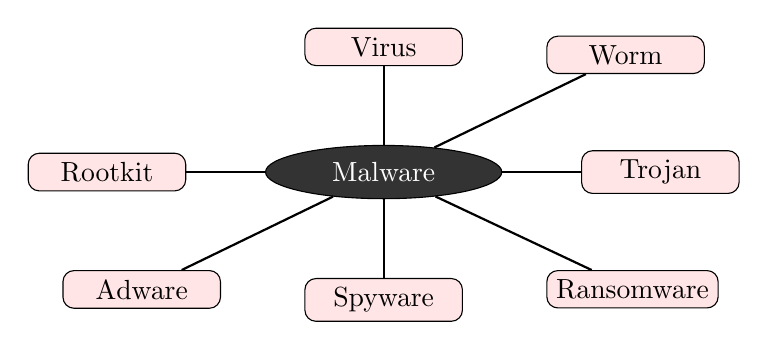
\begin{tikzpicture}[
    type/.style={draw, rectangle, rounded corners, fill=red!10, minimum width=2cm, align=center}
]
    \node [draw, ellipse, fill=black!80, text=white, minimum width=3cm] (center) {Malware};
    
    \node [type, above=of center] (virus) {Virus};
    \node [type, above right=of center] (worm) {Worm};
    \node [type, right=of center] (trojan) {Trojan};
    \node [type, below right=of center] (ransom) {Ransomware};
    \node [type, below=of center] (spy) {Spyware};
    \node [type, below left=of center] (ad) {Adware};
    \node [type, left=of center] (root) {Rootkit};
    
    \draw [thick] (center) -- (virus);
    \draw [thick] (center) -- (worm);
    \draw [thick] (center) -- (trojan);
    \draw [thick] (center) -- (ransom);
    \draw [thick] (center) -- (spy);
    \draw [thick] (center) -- (ad);
    \draw [thick] (center) -- (root);
\end{tikzpicture}
\end{answerdiagram}

\begin{answertable}{Malware Types and Effects}
\begin{tabulary}{\linewidth}{|L|L|L|L|}
\hline
\textbf{Type} & \textbf{Behavior} & \textbf{Effect} & \textbf{Example} \\ \hline
\keyword{Virus} & Attaches to files & File corruption & Boot sector virus \\ \hline
\keyword{Worm} & Self-replicating & Network congestion & Conficker worm \\ \hline
\keyword{Trojan} & Disguised malware & Data theft & Banking Trojans \\ \hline
\keyword{Ransomware} & Encrypts files & Data hostage & WannaCry \\ \hline
\keyword{Spyware} & Monitors activity & Privacy breach & Keyloggers \\ \hline
\keyword{Adware} & Shows unwanted ads & Performance degradation & Pop-up ads \\ \hline
\keyword{Rootkit} & Hides presence & System compromise & Kernel rootkits \\ \hline
\end{tabulary}
\end{answertable}

\textbf{Effects on Systems:}
\begin{itemize}
    \item \keyword{Performance}: Slow system response
    \item \keyword{Data}: Loss, corruption, or theft
    \item \keyword{Privacy}: Unauthorized monitoring
    \item \keyword{Financial}: Direct monetary loss
\end{itemize}

\textbf{Prevention Methods:}
\begin{itemize}
    \item Regular antivirus updates
    \item Safe browsing practices
    \item Email attachment caution
    \item System security patches
\end{itemize}
\end{solutionbox}

\begin{mnemonicbox}
\mnemonic{Viruses Worms Trojans Really Steal All Resources}
\end{mnemonicbox}

\questionmarks{2(a OR)}{3}{What is authentication? Explain different methods of authentication.}

\begin{solutionbox}
\textbf{Authentication Definition:}
Process of verifying user identity before granting system access.

\begin{answerdiagram}{Authentication Methods}
\begin{tikzpicture}[node distance=0.5cm, auto]
    \node [gtu block, fill=blue!10] (kn) {Something you KNOW\\(Password)};
    \node [gtu block, fill=green!10, right=of kn] (have) {Something you HAVE\\(Token)};
    \node [gtu block, fill=orange!10, right=of have] (are) {Something you ARE\\(Biometric)};
    
    \node [below=0.5cm of have] {\textbf{Multi-Factor Authentication (MFA)}};
\end{tikzpicture}
\end{answerdiagram}

\textbf{Authentication Methods:}
\begin{answertable}{Authentication Factors}
\begin{tabulary}{\linewidth}{|L|L|L|}
\hline
\textbf{Method} & \textbf{Description} & \textbf{Example} \\ \hline
\keyword{Password} & Something you know & PIN, passphrase \\ \hline
\keyword{Biometric} & Something you are & Fingerprint, iris \\ \hline
\keyword{Token} & Something you have & Smart card, USB key \\ \hline
\end{tabulary}
\end{answertable}

\begin{itemize}
    \item \keyword{Single-Factor}: Uses one authentication method
    \item \keyword{Multi-Factor}: Combines multiple methods
    \item \keyword{Two-Factor (2FA)}: Uses exactly two factors
\end{itemize}
\end{solutionbox}

\begin{mnemonicbox}
\mnemonic{Password Biometric Token Authentication}
\end{mnemonicbox}

\questionmarks{2(b OR)}{4}{Define: Trojans, Rootkit, Backdoors, Keylogger}

\begin{solutionbox}
\textbf{Malware Definitions:}

\begin{answertable}{Malware Definitions}
\begin{tabulary}{\linewidth}{|L|L|L|}
\hline
\textbf{Term} & \textbf{Definition} & \textbf{Characteristics} \\ \hline
\keyword{Trojans} & Malware disguised as legitimate software & Appears harmless, hidden payload \\ \hline
\keyword{Rootkit} & Software that hides malware presence & Deep system access, stealth operation \\ \hline
\keyword{Backdoors} & Unauthorized access method & Bypasses normal authentication \\ \hline
\keyword{Keylogger} & Records keyboard input & Captures passwords, sensitive data \\ \hline
\end{tabulary}
\end{answertable}

\begin{itemize}
    \item \keyword{Trojans}: Named after Greek Trojan Horse
    \item \keyword{Rootkit}: Operates at kernel level
    \item \keyword{Backdoors}: Can be hardware or software based
    \item \keyword{Keylogger}: Can be software or hardware device
\end{itemize}
\end{solutionbox}

\begin{mnemonicbox}
\mnemonic{Trojans Root Backdoors Keylog}
\end{mnemonicbox}

% Question 2(c OR) ... (continue in next chunk)


\questionmarks{2(c OR)}{7}{Explain Secure Socket Layer (SSL) and Transport Layer Security (TLS) protocols.}

\begin{solutionbox}
\textbf{SSL/TLS Protocol Evolution:}

\begin{answerdiagram}{SSL/TLS Handshake}
\begin{tikzpicture}[auto, >=latex, thick]
    \node [gtu state] (client) {Client};
    \node [gtu state, right=5cm of client] (server) {Server};
    
    % Sequence Diagram like flow
    \draw [->] (client.east) -- ++(0.5, -0.5) -- node [above, sloped, font=\footnotesize] {1. ClientHello} ($(server.west)+(0,-1)$);
    \draw [->] ($(server.west)+(0,-1.5)$) -- node [above, sloped, font=\footnotesize] {2. ServerHello + Cert} ($(client.east)+(0,-2)$);
    \draw [->] ($(client.east)+(0,-2.5)$) -- node [above, sloped, font=\footnotesize] {3. Key Exchange} ($(server.west)+(0,-3)$);
    \draw [->] ($(server.west)+(0,-3.5)$) -- node [above, sloped, font=\footnotesize] {4. Finished} ($(client.east)+(0,-4)$);
    
    \node [below=4.5cm of client, xshift=2.5cm, draw, dashed, fill=green!5] {Secure Channel Established};
\end{tikzpicture}
\end{answerdiagram}

\begin{answertable}{SSL/TLS Comparison}
\begin{tabulary}{\linewidth}{|L|L|L|L|}
\hline
\textbf{Version} & \textbf{Year} & \textbf{Status} & \textbf{Security Level} \\ \hline
\keyword{SSL 2.0} & 1995 & Deprecated & Weak \\ \hline
\keyword{SSL 3.0} & 1996 & Deprecated & Vulnerable \\ \hline
\keyword{TLS 1.0} & 1999 & Legacy & Limited \\ \hline
\keyword{TLS 1.2} & 2008 & Widely used & Good \\ \hline
\keyword{TLS 1.3} & 2018 & Current & Strong \\ \hline
\end{tabulary}
\end{answertable}

\textbf{Key Features:}
\begin{itemize}
    \item \keyword{Encryption}: Symmetric and asymmetric algorithms
    \item \keyword{Authentication}: Server and client verification
    \item \keyword{Integrity}: Message authentication codes
    \item \keyword{Forward Secrecy}: Session key protection
\end{itemize}

\textbf{Applications:}
\begin{itemize}
    \item HTTPS web browsing
    \item Email security (SMTPS)
    \item VPN connections
    \item Secure file transfers
\end{itemize}
\end{solutionbox}

\begin{mnemonicbox}
\mnemonic{TLS Encrypts All Network Traffic}
\end{mnemonicbox}

% Question 3
\questionmarks{3(a)}{3}{Explain in detail cybercrime and cybercriminal.}

\begin{solutionbox}
\textbf{Cybercrime Definition:}
Criminal activities conducted through computers or internet networks.

\begin{answerdiagram}{Cybercrime Overview}
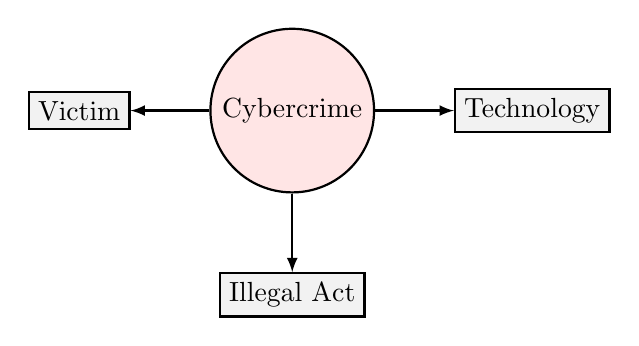
\begin{tikzpicture}[auto, >=latex, thick]
    \node [draw, circle, fill=red!10, align=center] (crime) {Cybercrime};
    \node [draw, rectangle, right=of crime, fill=gray!10] (tech) {Technology};
    \node [draw, rectangle, below=of crime, fill=gray!10] (illeg) {Illegal Act};
    \node [draw, rectangle, left=of crime, fill=gray!10] (vic) {Victim};
    
    \draw [->] (crime) -- (tech);
    \draw [->] (crime) -- (illeg);
    \draw [->] (crime) -- (vic);
\end{tikzpicture}
\end{answerdiagram}

\textbf{Cybercriminal Types:}
\begin{answertable}{Types of Cybercriminals}
\begin{tabulary}{\linewidth}{|L|L|L|L|}
\hline
\textbf{Type} & \textbf{Motivation} & \textbf{Skills} & \textbf{Target} \\ \hline
\keyword{Script Kiddies} & Fun/Fame & Low & Random \\ \hline
\keyword{Hacktivists} & Political/Social & Moderate & Organizations \\ \hline
\keyword{Cybercriminals} & Financial Gain & High & Individuals/Banks \\ \hline
\end{tabulary}
\end{answertable}

\begin{itemize}
    \item \keyword{Cybercrime}: Illegal activities using digital technology
    \item \keyword{Cybercriminal}: Person who commits cybercrimes
    \item \keyword{Impact}: Financial loss, privacy breach, system damage
\end{itemize}
\end{solutionbox}

\begin{mnemonicbox}
\mnemonic{Cyber Criminals Create Chaos}
\end{mnemonicbox}

\questionmarks{3(b)}{4}{Describe cyber stalking and cyber bullying in detail.}

\begin{solutionbox}
\textbf{Digital Harassment Comparison:}

\begin{answerdiagram}{Stalking vs Bullying}
\begin{tikzpicture}[auto, >=latex, thick]
    \node [gtu block, fill=orange!10, text width=3cm] (stalk) {Cyber Stalking\\(Targeted/Adult)};
    \node [gtu block, fill=purple!10, text width=3cm, right=of stalk] (bully) {Cyber Bullying\\(Broad/Minor)};
    
    \draw [<->] (stalk) -- node {Both Harass} (bully);
\end{tikzpicture}
\end{answerdiagram}

\begin{answertable}{Stalking vs Bullying}
\begin{tabulary}{\linewidth}{|L|L|L|}
\hline
\textbf{Aspect} & \textbf{Cyber Stalking} & \textbf{Cyber Bullying} \\ \hline
\keyword{Target} & Specific individual & Often minors \\ \hline
\keyword{Duration} & Persistent, long-term & Can be episodic \\ \hline
\keyword{Intent} & Intimidation, control & Harassment, humiliation \\ \hline
\keyword{Platform} & Social media, email & Schools, gaming platforms \\ \hline
\end{tabulary}
\end{answertable}

\textbf{Cyber Stalking Characteristics:}
\begin{itemize}
    \item Persistent unwanted contact
    \item Monitoring victim's online activity
    \item Threatening messages or behavior
    \item Identity theft or impersonation
\end{itemize}

\textbf{Cyber Bullying Forms:}
\begin{itemize}
    \item Public humiliation online
    \item Exclusion from digital groups
    \item Spreading false information
    \item Sharing private content without consent
\end{itemize}

\textbf{Prevention Measures:}
\begin{itemize}
    \item Privacy settings on social media
    \item Reporting harassment to platforms
    \item Legal action when necessary
    \item Digital literacy education
\end{itemize}
\end{solutionbox}

\begin{mnemonicbox}
\mnemonic{Stop Bullying, Report Stalking}
\end{mnemonicbox}

\questionmarks{3(c)}{7}{Explain Property based classification in cybercrime.}

\begin{solutionbox}
\textbf{Property-Based Cybercrime Categories:}

\begin{answerdiagram}{Property-Based Cybercrime}
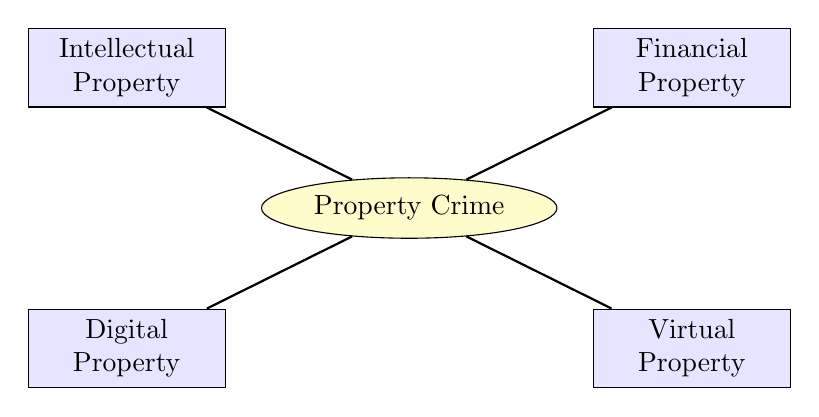
\begin{tikzpicture}[
    prop/.style={draw, rectangle, fill=blue!10, minimum width=2.5cm, minimum height=1cm, align=center}
]
    \node [draw, ellipse, fill=yellow!20] (center) {Property Crime};
    
    \node [prop, above left=of center] (ip) {Intellectual\\Property};
    \node [prop, above right=of center] (fin) {Financial\\Property};
    \node [prop, below left=of center] (dig) {Digital\\Property};
    \node [prop, below right=of center] (virt) {Virtual\\Property};
    
    \draw [thick] (center) -- (ip);
    \draw [thick] (center) -- (fin);
    \draw [thick] (center) -- (dig);
    \draw [thick] (center) -- (virt);
\end{tikzpicture}
\end{answerdiagram}

\begin{answertable}{Property Crime Classification}
\begin{tabulary}{\linewidth}{|L|L|L|L|}
\hline
\textbf{Category} & \textbf{Crime Type} & \textbf{Description} & \textbf{Example} \\ \hline
\keyword{Intellectual Property} & Copyright infringement & Unauthorized use of copyrighted material & Software piracy \\ \hline
\keyword{Financial Property} & Credit card fraud & Unauthorized use of financial information & Online shopping fraud \\ \hline
\keyword{Digital Property} & Data theft & Stealing digital information & Database breaches \\ \hline
\keyword{Virtual Property} & Gaming asset theft & Stealing virtual goods & Online game currency theft \\ \hline
\end{tabulary}
\end{answertable}

\textbf{Legal Aspects:}
\begin{itemize}
    \item \keyword{Copyright Laws}: Protect creative works
    \item \keyword{Trademark Laws}: Protect brand identity
    \item \keyword{Patent Laws}: Protect inventions
    \item \keyword{Trade Secret Laws}: Protect confidential information
\end{itemize}

\textbf{Impact on Economy:}
\begin{itemize}
    \item Revenue loss for legitimate businesses
    \item Reduced innovation incentives
    \item Consumer trust erosion
    \item Legal enforcement costs
\end{itemize}

\textbf{Prevention Strategies:}
\begin{itemize}
    \item Digital rights management (DRM)
    \item Watermarking and tracking
    \item Legal enforcement mechanisms
    \item Public awareness campaigns
\end{itemize}
\end{solutionbox}

\begin{mnemonicbox}
\mnemonic{Property Protection Prevents Piracy}
\end{mnemonicbox}

\questionmarks{3(a OR)}{3}{Explain Data diddling.}

\begin{solutionbox}
\textbf{Data Diddling Definition:}
Unauthorized alteration of data before or during input into computer systems.

\begin{answerdiagram}{Data Diddling Process}
\begin{tikzpicture}[auto, >=latex, thick]
    \node [gtu block] (source) {Source Doc};
    \node [gtu block, right=of source, fill=red!20] (diddle) {Alteration\\(Diddling)};
    \node [gtu block, right=of diddle] (input) {System Input};
    \node [gtu block, right=of input] (db) {Database};
    
    \draw [gtu arrow] (source) -- (diddle);
    \draw [gtu arrow] (diddle) -- (input);
    \draw [gtu arrow] (input) -- (db);
    
    \node [below=of diddle, font=\small] {Changes happen here};
\end{tikzpicture}
\end{answerdiagram}

\textbf{Characteristics:}
\begin{answertable}{Data Diddling Characteristics}
\begin{tabulary}{\linewidth}{|L|L|}
\hline
\textbf{Aspect} & \textbf{Description} \\ \hline
\keyword{Method} & Changing data values \\ \hline
\keyword{Timing} & Before system processing \\ \hline
\keyword{Detection} & Often difficult to identify \\ \hline
\end{tabulary}
\end{answertable}

\begin{itemize}
    \item \keyword{Examples}: Changing salary figures, altering exam scores
    \item \keyword{Target}: Input data during entry process
    \item \keyword{Impact}: Financial loss, incorrect records
\end{itemize}
\end{solutionbox}

\begin{mnemonicbox}
\mnemonic{Data Diddling Damages Databases}
\end{mnemonicbox}

\questionmarks{3(b OR)}{4}{Explain cyber spying and cyber terrorism.}

\begin{solutionbox}
\textbf{Cyber Threats Comparison:}

\begin{answertable}{Spying vs Terrorism}
\begin{tabulary}{\linewidth}{|L|L|L|}
\hline
\textbf{Aspect} & \textbf{Cyber Spying} & \textbf{Cyber Terrorism} \\ \hline
\keyword{Purpose} & Information gathering & Causing fear/disruption \\ \hline
\keyword{Target} & Government, corporations & Critical infrastructure \\ \hline
\keyword{Methods} & Stealth infiltration & Destructive attacks \\ \hline
\keyword{Impact} & Intelligence loss & Public safety risk \\ \hline
\end{tabulary}
\end{answertable}

\textbf{Cyber Spying Activities:}
\begin{itemize}
    \item Corporate espionage
    \item Government surveillance
    \item Trade secret theft
    \item Personal information gathering
\end{itemize}

\textbf{Cyber Terrorism Methods:}
\begin{itemize}
    \item Infrastructure attacks
    \item Mass disruption campaigns
    \item Psychological warfare
    \item Economic damage
\end{itemize}

\textbf{Prevention Measures:}
\begin{itemize}
    \item Network security monitoring
    \item Incident response planning
    \item International cooperation
    \item Public-private partnerships
\end{itemize}
\end{solutionbox}

\begin{mnemonicbox}
\mnemonic{Spies Steal, Terrorists Terror}
\end{mnemonicbox}

\questionmarks{3(c OR)}{7}{Explain the role of digital signatures and digital certificates in cybersecurity.}

\begin{solutionbox}
\textbf{Digital Security Components:}

\begin{answerdiagram}{Digital Signature Process}
\begin{tikzpicture}[auto, >=latex, thick, node distance=1.5cm]
    \node [gtu block, fill=white] (doc) {Document};
    \node [gtu block, right=of doc, fill=orange!10] (hash) {Hash Function};
    \node [gtu block, right=of hash, fill=yellow!10] (digest) {Digest};
    \node [gtu block, right=of digest, fill=red!10] (encrypt) {Encrypt w/\\Private Key};
    \node [gtu block, right=of encrypt, fill=green!10] (sig) {Digital\\Signature};
    
    \draw [gtu arrow] (doc) -- (hash);
    \draw [gtu arrow] (hash) -- (digest);
    \draw [gtu arrow] (digest) -- (encrypt);
    \draw [gtu arrow] (encrypt) -- (sig);
\end{tikzpicture}
\end{answerdiagram}

\begin{answertable}{Digital Security Components}
\begin{tabulary}{\linewidth}{|L|L|L|L|}
\hline
\textbf{Component} & \textbf{Purpose} & \textbf{Function} & \textbf{Benefit} \\ \hline
\keyword{Digital Signature} & Authentication & Proves sender identity & Non-repudiation \\ \hline
\keyword{Digital Certificate} & Verification & Validates public keys & Trust establishment \\ \hline
\end{tabulary}
\end{answertable}

\textbf{Digital Certificate Components:}
\begin{itemize}
    \item \keyword{Subject Information}: Certificate owner details
    \item \keyword{Public Key}: For encryption/verification
    \item \keyword{Digital Signature}: CA's signature
    \item \keyword{Validity Period}: Certificate expiration date
\end{itemize}

\textbf{Certificate Authority (CA) Role:}
\begin{itemize}
    \item Issues digital certificates
    \item Verifies identity before issuance
    \item Maintains certificate revocation lists
    \item Provides trust infrastructure
\end{itemize}

\textbf{Security Benefits:}
\begin{itemize}
    \item \keyword{Authentication}: Verifies sender identity
    \item \keyword{Integrity}: Ensures data hasn't been modified
    \item \keyword{Non-repudiation}: Prevents denial of actions
    \item \keyword{Confidentiality}: Enables secure communication
\end{itemize}
\end{solutionbox}

\begin{mnemonicbox}
\mnemonic{Digital Signatures Authenticate Documents Securely}
\end{mnemonicbox}

% Question 4
\questionmarks{4(a)}{3}{What is Hacking? List out types of Hackers.}

\begin{solutionbox}
\textbf{Hacking Definition:}
Unauthorized access to computer systems or networks to exploit vulnerabilities.

\begin{answerdiagram}{Hacker Types}
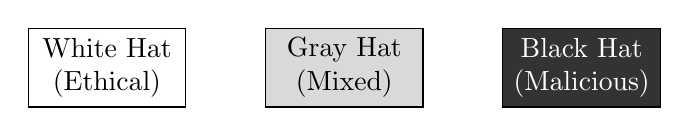
\begin{tikzpicture}[
    hat/.style={draw, rectangle, minimum width=2cm, minimum height=1cm, align=center}
]
    \node [hat, fill=white] (white) {White Hat\\(Ethical)};
    \node [hat, right=of white, fill=gray!30] (gray) {Gray Hat\\(Mixed)};
    \node [hat, right=of gray, fill=black!80, text=white] (black) {Black Hat\\(Malicious)};
\end{tikzpicture}
\end{answerdiagram}

\textbf{Hacker Classifications:}
\begin{answertable}{Types of Hackers}
\begin{tabulary}{\linewidth}{|L|L|L|}
\hline
\textbf{Type} & \textbf{Intent} & \textbf{Legal Status} \\ \hline
\keyword{White Hat} & Security improvement & Legal \\ \hline
\keyword{Black Hat} & Malicious activities & Illegal \\ \hline
\keyword{Gray Hat} & Mixed motivations & Questionable \\ \hline
\end{tabulary}
\end{answertable}
\end{solutionbox}

\begin{mnemonicbox}
\mnemonic{White Good, Black Bad, Gray Questionable}
\end{mnemonicbox}

\questionmarks{4(b)}{4}{Explain Vulnerability and 0-Day terminology of Hacking.}

\begin{solutionbox}
\textbf{Security Terminology:}

\begin{answertable}{Vulnerability vs 0-Day}
\begin{tabulary}{\linewidth}{|L|L|L|L|}
\hline
\textbf{Term} & \textbf{Definition} & \textbf{Risk Level} & \textbf{Example} \\ \hline
\keyword{Vulnerability} & System weakness & Varies & Unpatched software \\ \hline
\keyword{0-Day} & Unknown vulnerability & Critical & Undiscovered flaw \\ \hline
\end{tabulary}
\end{answertable}

\textbf{Vulnerability Characteristics:}
\begin{itemize}
    \item Discovery through security testing
    \item Disclosure to vendors
    \item Patching via updates
\end{itemize}

\textbf{0-Day Attack Process:}
\begin{enumerate}
    \item Hacker discovers unknown vulnerability
    \item Exploits flaw before vendor awareness
    \item No available patches or defenses
    \item High success rate due to surprise element
\end{enumerate}
\end{solutionbox}

\begin{mnemonicbox}
\mnemonic{Vulnerabilities Need Patches, Zero-Days Need Vigilance}
\end{mnemonicbox}

\questionmarks{4(c)}{7}{Explain Five Steps of Hacking.}

\begin{solutionbox}
\textbf{Hacking Methodology:}

\begin{answerdiagram}{Hacking Steps}
\begin{tikzpicture}[
    step/.style={gtu block, minimum width=2.5cm}
]
    \node [step, fill=blue!10] (recon) {1. Reconnaissance};
    \node [step, right=0.5cm of recon, fill=green!10] (scan) {2. Scanning};
    \node [step, right=0.5cm of scan, fill=orange!10] (gain) {3. Gaining Access};
    
    \node [step, below=of recon, xshift=1.5cm, fill=red!10] (maint) {4. Maintaining Access};
    \node [step, right=0.5cm of maint, fill=gray!10] (cover) {5. Covering Tracks};
    
    \draw [gtu arrow] (recon) -- (scan);
    \draw [gtu arrow] (scan) -- (gain);
    \draw [gtu arrow] (gain) -- (maint);
    \draw [gtu arrow] (maint) -- (cover);
\end{tikzpicture}
\end{answerdiagram}

\textbf{Detailed Steps:}
\begin{answertable}{Hacking Phases}
\begin{tabulary}{\linewidth}{|L|L|L|L|}
\hline
\textbf{Step} & \textbf{Description} & \textbf{Tools/Methods} & \textbf{Objective} \\ \hline
\keyword{Reconnaissance} & Information gathering & Google dorking, Social media & Target profiling \\ \hline
\keyword{Scanning} & System enumeration & Nmap, Nessus & Vulnerability identification \\ \hline
\keyword{Gaining Access} & Exploit vulnerabilities & Metasploit, Custom exploits & System compromise \\ \hline
\keyword{Maintaining Access} & Persistent presence & Backdoors, Rootkits & Long-term control \\ \hline
\keyword{Covering Tracks} & Evidence removal & Log cleaning, File deletion & Avoid detection \\ \hline
\end{tabulary}
\end{answertable}

\textbf{Techniques Breakdown:}
\begin{itemize}
    \item \keyword{Reconnaissance}: Passive vs Active information gathering
    \item \keyword{Scanning}: Port scanning, vulnerability scanning
    \item \keyword{Access Methods}: Password attacks, exploits, social engineering
    \item \keyword{Persistence}: Backdoors, user accounts, scheduled tasks
    \item \keyword{Covering Tracks}: Log wiping, encryption, timestamp modification
\end{itemize}
\end{solutionbox}

\begin{mnemonicbox}
\mnemonic{Reconnaissance Scans Generate Access, Maintain Coverage}
\end{mnemonicbox}

\questionmarks{4(a OR)}{3}{Explain any three basic commands of Kali Linux with suitable example.}

\begin{solutionbox}
\textbf{Essential Kali Linux Commands:}

\begin{answertable}{Kali Commands}
\begin{tabulary}{\linewidth}{|L|L|L|}
\hline
\textbf{Command} & \textbf{Function} & \textbf{Example} \\ \hline
\keyword{nmap} & Network scanning & \code{nmap -sS 192.168.1.1} \\ \hline
\keyword{netcat} & Network communication & \code{nc -l -p 1234} \\ \hline
\keyword{hydra} & Password cracking & \code{hydra -l admin -P pass.txt ssh://target} \\ \hline
\end{tabulary}
\end{answertable}

\begin{itemize}
    \item \keyword{Nmap}: Discovers hosts and services on network
    \item \keyword{Netcat}: Creates network connections for data transfer
    \item \keyword{Hydra}: Performs brute-force password attacks
\end{itemize}
\end{solutionbox}

\begin{mnemonicbox}
\mnemonic{Network Map, Connect, Crack}
\end{mnemonicbox}

\questionmarks{4(b OR)}{4}{Describe Session Hijacking in detail.}

\begin{solutionbox}
\textbf{Session Hijacking Overview:}
Attack where attacker takes over legitimate user's session.

\begin{answerdiagram}{Session Hijacking}
\begin{tikzpicture}[auto, >=latex, thick]
    \node [gtu state] (client) {User};
    \node [gtu state, right=4cm of client] (server) {Server};
    \node [gtu state, below=2cm of client, fill=red!20] (attacker) {Attacker};
    
    \draw [thick, blue] (client) -- node[above] {Valid Session} (server);
    \draw [dashed, red, ->] (attacker) -- node[right, font=\footnotesize] {Steals Session ID} (client);
    \draw [thick, red, ->] (attacker) to[bend right=20] node[below, font=\footnotesize] {Impersonates User} (server);
\end{tikzpicture}
\end{answerdiagram}

\begin{answertable}{Hijacking Types}
\begin{tabulary}{\linewidth}{|L|L|L|}
\hline
\textbf{Type} & \textbf{Method} & \textbf{Prevention} \\ \hline
\keyword{Active} & Takes over session & Strong session management \\ \hline
\keyword{Passive} & Monitors session & Encryption (HTTPS) \\ \hline
\keyword{Network-level} & TCP hijacking & Secure protocols \\ \hline
\keyword{Application-level} & Cookie theft & Secure cookie attributes \\ \hline
\end{tabulary}
\end{answertable}

\textbf{Prevention Measures:}
\begin{itemize}
    \item Use HTTPS for all communications
    \item Implement secure session management
    \item Set secure cookie attributes
    \item Monitor for suspicious activity
\end{itemize}
\end{solutionbox}

\begin{mnemonicbox}
\mnemonic{Sessions Hijacked Need Secure Handling}
\end{mnemonicbox}

\questionmarks{4(c OR)}{7}{Explain how Virtual Private Networks (VPNs) create secure, encrypted connections over public networks.}

\begin{solutionbox}
\textbf{VPN Architecture:}

\begin{answerdiagram}{VPN Architecture}
\begin{tikzpicture}[auto, >=latex, thick]
    \node [gtu block] (user) {User Device};
    \node [draw, cloud, cloud puffs=10, right=1.5cm of user, minimum width=3cm] (internet) {Internet};
    \node [gtu block, right=1.5cm of internet] (server) {VPN Server};
    
    % Tunnel
    \draw [double, double distance=2pt, dashed, blue] (user) -- (server);
    \node [above=0.2cm of internet, text=blue] {Encrypted Tunnel};
    
    % Connections
    \node [right=1cm of server] (dest) {Destination};
    \draw [->] (server) -- (dest);
\end{tikzpicture}
\end{answerdiagram}

\begin{answertable}{VPN Protocols}
\begin{tabulary}{\linewidth}{|L|L|L|L|}
\hline
\textbf{Protocol} & \textbf{Security} & \textbf{Speed} & \textbf{Use Case} \\ \hline
\keyword{OpenVPN} & High & Good & General purpose \\ \hline
\keyword{IPSec} & Very High & Moderate & Enterprise \\ \hline
\keyword{WireGuard} & High & Excellent & Modern solution \\ \hline
\keyword{PPTP} & Low & Fast & Legacy (deprecated) \\ \hline
\end{tabulary}
\end{answertable}

\textbf{VPN Working Process:}
\begin{enumerate}
    \item \keyword{Connection}: Client connects to VPN server
    \item \keyword{Authentication}: User credentials verified
    \item \keyword{Tunnel Creation}: Encrypted pathway established
    \item \keyword{Data Encryption}: All traffic encrypted
    \item \keyword{Routing/Decryption}: Traffic routed/decrypted at destination
\end{enumerate}

\textbf{Benefits:}
\begin{itemize}
    \item \keyword{Data Protection}: Encryption prevents eavesdropping
    \item \keyword{Privacy}: IP address masking
    \item \keyword{Access Control}: Authenticate before connection
    \item \keyword{Bypass Restrictions}: Access geo-blocked content
\end{itemize}
\end{solutionbox}

\begin{mnemonicbox}
\mnemonic{VPNs Provide Network Privacy}
\end{mnemonicbox}


% Question 5
\questionmarks{5(a)}{3}{Explain Network forensics.}

\begin{solutionbox}
\textbf{Network Forensics Definition:}
Investigation of network traffic to detect and analyze security incidents.

\begin{answerdiagram}{Network Forensics Process}
\begin{tikzpicture}[auto, >=latex, thick]
    \node [gtu block, fill=blue!10] (cap) {Traffic Capture};
    \node [gtu block, right=of cap, fill=yellow!10] (ana) {Analysis};
    \node [gtu block, right=of ana, fill=green!10] (evi) {Evidence};
    
    \draw [gtu arrow] (cap) -- (ana);
    \draw [gtu arrow] (ana) -- (evi);
    
    \node [below=0.5cm of ana, font=\small] {Wireshark, tcpdump};
\end{tikzpicture}
\end{answerdiagram}

\textbf{Key Components:}
\begin{answertable}{Network Forensics Components}
\begin{tabulary}{\linewidth}{|L|L|L|}
\hline
\textbf{Component} & \textbf{Purpose} & \textbf{Tools} \\ \hline
\keyword{Traffic Capture} & Record network data & Wireshark, tcpdump \\ \hline
\keyword{Analysis} & Examine patterns & NetworkMiner, Snort \\ \hline
\keyword{Evidence} & Document findings & Forensic reports \\ \hline
\end{tabulary}
\end{answertable}

\begin{itemize}
    \item \keyword{Scope}: Analyzes packets, flows, and network behavior
    \item \keyword{Objective}: Identify security breaches and attack patterns
    \item \keyword{Challenge}: Large data volumes and real-time processing
\end{itemize}
\end{solutionbox}

\begin{mnemonicbox}
\mnemonic{Network Forensics Finds Facts}
\end{mnemonicbox}

\questionmarks{5(b)}{4}{Explain why CCTV plays an important role as evidence in digital forensics investigations.}

\begin{solutionbox}
\textbf{CCTV in Digital Forensics:}

\begin{answerdiagram}{CCTV Evidence}
\begin{tikzpicture}[auto, >=latex, thick]
    \node [gtu block] (cam) {CCTV Camera};
    \node [gtu block, right=of cam] (dvr) {DVR/NVR};
    \node [gtu block, right=of dvr] (forensic) {Forensic\\Analysis};
    \node [gtu block, right=of forensic, fill=green!10] (court) {Court\\Evidence};
    
    \draw [gtu arrow] (cam) -- (dvr);
    \draw [gtu arrow] (dvr) -- (forensic);
    \draw [gtu arrow] (forensic) -- (court);
\end{tikzpicture}
\end{answerdiagram}

\begin{answertable}{CCTV Evidence Value}
\begin{tabulary}{\linewidth}{|L|L|L|}
\hline
\textbf{Aspect} & \textbf{Importance} & \textbf{Value} \\ \hline
\keyword{Visual Evidence} & Direct observation & High credibility \\ \hline
\keyword{Timeline} & Time-stamped records & Event correlation \\ \hline
\keyword{Digital Format} & Easy to analyze & Metadata extraction \\ \hline
\keyword{Backup} & Multiple copies & Evidence preservation \\ \hline
\end{tabulary}
\end{answertable}

\textbf{Evidence Value:}
\begin{itemize}
    \item \keyword{Corroboration}: Supports other digital evidence
    \item \keyword{Timeline}: Establishes sequence of events
    \item \keyword{Identity}: May reveal perpetrator identity
    \item \keyword{Context}: Shows physical environment during incident
\end{itemize}

\textbf{Forensic Considerations:}
\begin{itemize}
    \item \keyword{Chain of Custody}: Proper evidence handling
    \item \keyword{Authentication}: Verify video integrity
    \item \keyword{Analysis}: Enhancement and interpretation
    \item \keyword{Legal Admissibility}: Court-acceptable format
\end{itemize}
\end{solutionbox}

\begin{mnemonicbox}
\mnemonic{CCTV Captures Criminal Conduct Clearly}
\end{mnemonicbox}

\questionmarks{5(c)}{7}{Explain phases of Digital forensic investigation.}

\begin{solutionbox}
\textbf{Digital Forensics Investigation Phases:}

\begin{answerdiagram}{Digital Forensics Phases}
\begin{tikzpicture}[
    phase/.style={gtu block, minimum width=3cm}
]
    \node [phase, fill=blue!10] (id) {1. Identification};
    \node [phase, right=of id, fill=cyan!10] (pres) {2. Preservation};
    \node [phase, right=of pres, fill=green!10] (col) {3. Collection};
    
    \node [phase, below=of id, fill=yellow!10] (exam) {4. Examination};
    \node [phase, right=of exam, fill=orange!10] (ana) {5. Analysis};
    \node [phase, right=of ana, fill=red!10] (present) {6. Presentation};
    
    \draw [gtu arrow] (id) -- (pres);
    \draw [gtu arrow] (pres) -- (col);
    \draw [gtu arrow] (col) -- (exam); % logical flow wrapping
    \draw [gtu arrow] (exam) -- (ana);
    \draw [gtu arrow] (ana) -- (present);
\end{tikzpicture}
\end{answerdiagram}

\begin{answertable}{Investigation Phases}
\begin{tabulary}{\linewidth}{|L|L|L|L|}
\hline
\textbf{Phase} & \textbf{Activities} & \textbf{Tools} & \textbf{Objective} \\ \hline
\keyword{Identification} & Recognize potential evidence & Visual inspection & Scope definition \\ \hline
\keyword{Preservation} & Prevent evidence contamination & Write blockers & Evidence integrity \\ \hline
\keyword{Collection} & Acquire digital evidence & Forensic imaging & Complete data capture \\ \hline
\keyword{Examination} & Extract relevant data & Autopsy, FTK & Data recovery \\ \hline
\keyword{Analysis} & Interpret findings & Timeline tools & Pattern identification \\ \hline
\keyword{Presentation} & Document results & Report generators & Legal presentation \\ \hline
\end{tabulary}
\end{answertable}

\textbf{Phase 1 - Identification:}
\begin{itemize}
    \item Survey the scene and identify evidence sources
    \item Document initial observations and establish scope
\end{itemize}

\textbf{Phase 2 - Preservation:}
\begin{itemize}
    \item Secure crime scene and prevent contamination
    \item Use write-protection mechanisms
\end{itemize}

\textbf{Phase 3 - Collection:}
\begin{itemize}
    \item Create forensic images and maintain chain of custody
    \item Generate hash values for verification
\end{itemize}

\textbf{Phase 4 - Examination:}
\begin{itemize}
    \item Extract file systems and recover deleted data
    \item Identify relevant files
\end{itemize}

\textbf{Phase 5 - Analysis:}
\begin{itemize}
    \item Correlate evidence and reconstruct events
    \item Identify patterns and form conclusions
\end{itemize}

\textbf{Phase 6 - Presentation:}
\begin{itemize}
    \item Prepare detailed reports and visual presentations
    \item Explain technical findings for legal proceedings
\end{itemize}

\textbf{Quality Assurance:}
\begin{itemize}
    \item \keyword{Documentation}, \keyword{Validation}, \keyword{Reproducibility}, \keyword{Legal Compliance}
\end{itemize}
\end{solutionbox}

\begin{mnemonicbox}
\mnemonic{Investigators Preserve, Collect, Examine, Analyze, Present}
\end{mnemonicbox}

\questionmarks{5(a OR)}{3}{List applications of microcontrollers in various fields related to cybersecurity.}

\begin{solutionbox}
\textbf{Microcontroller Security Applications:}

\begin{answerdiagram}{Microcontroller Security}
\begin{tikzpicture}[auto, >=latex, thick]
    \node [gtu block] (mcu) {Microcontroller};
    \node [gtu block, above right=of mcu] (iot) {IoT Security};
    \node [gtu block, right=of mcu] (access) {Access Control};
    \node [gtu block, below right=of mcu] (net) {Network Security};
    
    \draw [gtu arrow] (mcu) -- (iot);
    \draw [gtu arrow] (mcu) -- (access);
    \draw [gtu arrow] (mcu) -- (net);
\end{tikzpicture}
\end{answerdiagram}

\begin{answertable}{Microcontroller Applications}
\begin{tabulary}{\linewidth}{|L|L|L|}
\hline
\textbf{Field} & \textbf{Application} & \textbf{Security Function} \\ \hline
\keyword{IoT Security} & Smart home devices & Authentication, encryption \\ \hline
\keyword{Access Control} & Key cards, biometric & Identity verification \\ \hline
\keyword{Network Security} & Hardware firewalls & Packet filtering \\ \hline
\end{tabulary}
\end{answertable}

\begin{itemize}
    \item \keyword{Smart Cards}: Secure authentication tokens
    \item \keyword{HSM (Hardware Security Modules)}: Cryptographic processing
    \item \keyword{Embedded Systems}: Secure boot, tamper detection
\end{itemize}
\end{solutionbox}

\begin{mnemonicbox}
\mnemonic{Microcontrollers Manage Multiple Security Functions}
\end{mnemonicbox}

\questionmarks{5(b OR)}{4}{Explain the importance of port scanning in ethical hacking.}

\begin{solutionbox}
\textbf{Port Scanning in Ethical Hacking:}

\begin{answerdiagram}{Port Scanning Benefits}
\begin{tikzpicture}[auto, >=latex, thick]
    \node [gtu block, circular drop shadow, fill=gray!10] (scan) {Port Scanning};
    
    \node [gtu block, above right=of scan] (vuln) {Find\\Vulnerabilities};
    \node [gtu block, below right=of scan] (serv) {Discover\\Services};
    \node [gtu block, right=of scan] (map) {Map\\Network};
    
    \draw [gtu arrow] (scan) -- (vuln);
    \draw [gtu arrow] (scan) -- (serv);
    \draw [gtu arrow] (scan) -- (map);
\end{tikzpicture}
\end{answerdiagram}

\begin{answertable}{Port Scanning Importance}
\begin{tabulary}{\linewidth}{|L|L|L|}
\hline
\textbf{Aspect} & \textbf{Importance} & \textbf{Benefit} \\ \hline
\keyword{Service Discovery} & Identify running services & Attack surface mapping \\ \hline
\keyword{Vulnerability Assessment} & Find open ports & Security gap identification \\ \hline
\keyword{Network Mapping} & Understand topology & Infrastructure analysis \\ \hline
\keyword{Security Testing} & Validate configurations & Compliance verification \\ \hline
\end{tabulary}
\end{answertable}

\textbf{Port Scanning Techniques:}
\begin{itemize}
    \item \keyword{TCP Connect}: Full connection establishment
    \item \keyword{SYN Scan}: Stealth scanning method
    \item \keyword{UDP Scan}: User Datagram Protocol scanning
    \item \keyword{Service Detection}: Identify service versions
\end{itemize}

\textbf{Ethical Considerations:}
\begin{itemize}
    \item \keyword{Authorization}: Obtain proper permissions
    \item \keyword{Scope}: Stay within defined boundaries
    \item \keyword{Documentation}: Record all activities
    \item \keyword{Reporting}: Provide detailed findings
\end{itemize}
\end{solutionbox}

\begin{mnemonicbox}
\mnemonic{Port Scanning Provides Security Insights}
\end{mnemonicbox}

\questionmarks{5(c OR)}{7}{Describe the process of conducting a vulnerability assessment using Kali Linux tools.}

\begin{solutionbox}
\textbf{Vulnerability Assessment Process with Kali:}

\begin{answerdiagram}{Assessment Process}
\begin{tikzpicture}[auto, >=latex, thick]
    \node [gtu block] (recon) {Recon};
    \node [gtu block, right=of recon] (port) {Port Scan};
    \node [gtu block, right=of port] (vuln) {Vuln Scan};
    \node [gtu block, right=of vuln] (man) {Manual};
    \node [gtu block, right=of man] (report) {Report};
    
    \draw [gtu arrow] (recon) -- (port);
    \draw [gtu arrow] (port) -- (vuln);
    \draw [gtu arrow] (vuln) -- (man);
    \draw [gtu arrow] (man) -- (report);
    
    \node [below=0.2cm of recon, font=\tiny] {Nmap};
    \node [below=0.2cm of port, font=\tiny] {Nmap/Masscan};
    \node [below=0.2cm of vuln, font=\tiny] {OpenVAS};
    \node [below=0.2cm of man, font=\tiny] {Metasploit};
\end{tikzpicture}
\end{answerdiagram}

\textbf{Step-by-Step Process \& Tools:}
\begin{answertable}{Assessment Steps}
\begin{tabulary}{\linewidth}{|L|L|L|L|}
\hline
\textbf{Step} & \textbf{Kali Tool} & \textbf{Command Example} & \textbf{Purpose} \\ \hline
\keyword{Reconnaissance} & Nmap & \code{nmap -sn 192.168.1.0/24} & Host discovery \\ \hline
\keyword{Port Scanning} & Nmap & \code{nmap -sS -O target} & Open port identification \\ \hline
\keyword{Service Enumeration} & Nmap & \code{nmap -sV target} & Service version detection \\ \hline
\keyword{Vulnerability Scan} & OpenVAS & \code{openvas-start} & Automated detection \\ \hline
\keyword{Web App Test} & Nikto & \code{nikto -h target} & Web vulnerability scanning \\ \hline
\end{tabulary}
\end{answertable}

\textbf{Detailed Phases:}
\begin{itemize}
    \item \keyword{Phase 1 - Target Identification}: Map network, identify live hosts.
    \item \keyword{Phase 2 - Port/Service Analysis}: Find open ports and service versions.
    \item \keyword{Phase 3 - Automated Scanning}: Use OpenVAS/Nessus for automated checks.
    \item \keyword{Phase 4 - Manual Testing}: Verify findings, test specific flaws (SQLi, XSS).
    \item \keyword{Phase 5 - Reporting}: Document findings, risk ratings, and remediation.
\end{itemize}

\textbf{Common Kali Tools:}
\begin{itemize}
    \item \keyword{Nmap}: Network scanning
    \item \keyword{OpenVAS}: Vulnerability scanning
    \item \keyword{Nikto}: Web server scanning
    \item \keyword{Metasploit}: Validation/Exploitation
    \item \keyword{Burp Suite}: Web proxy for manual testing
\end{itemize}

\textbf{Best Practices:}
\begin{itemize}
    \item \keyword{Authorization}: Always obtain written permission
    \item \keyword{Documentation}: Maintain detailed logs
    \item \keyword{Minimal Impact}: Avoid disrupting production
    \item \keyword{Confidentiality}: Protect discovered data
\end{itemize}
\end{solutionbox}

\begin{mnemonicbox}
\mnemonic{Vulnerability Assessment Validates Application Security}
\end{mnemonicbox}

\end{document}


